%% Supplementary material for the pyRMT method paper -- Elsevier (elsarticle).
%% Build:  pdflatex supplementary ; bibtex supplementary ; pdflatex supplementary ; pdflatex supplementary
\documentclass[final,3p,times]{elsarticle}

\usepackage[T1]{fontenc}
\usepackage{lmodern}
\usepackage{amsmath,amssymb,bm}
\usepackage{mathtools}
\usepackage{graphicx}
\usepackage{booktabs}
\usepackage[hidelinks]{hyperref}
\usepackage{cleveref}
\usepackage{xcolor}

% ---- notation (shared with the main text) ----
\newcommand{\uv}{\bm{u}}
\newcommand{\xiv}{\bm{\xi}}
\newcommand{\be}{\bm{b}_e}
\newcommand{\Ften}{\bm{F}}
\newcommand{\It}{\bm{I}}
\newcommand{\psib}{\bm{\psi}}
\newcommand{\grad}{\nabla}
\newcommand{\dt}{\Delta t}
\newcommand{\dx}{\Delta x}

% ---- supplementary numbering: prefix everything with "S" ----
\renewcommand{\thesection}{S\arabic{section}}
\renewcommand{\thefigure}{S\arabic{figure}}
\renewcommand{\thetable}{S\arabic{table}}
\renewcommand{\theequation}{S\arabic{equation}}

\begin{document}

\begin{frontmatter}
\title{Supplementary material for ``A semi-implicit log-conformation Reference Map
Technique for incompressible viscoelastic fluid--structure interaction''}
\author[bu]{Saman Seifi}\ead{samansei@bu.edu}
\address[bu]{Department of Mechanical Engineering, Boston University,
Boston, MA 02215, USA}
\end{frontmatter}

\noindent This supplement collects the fluid-solver and time-integrator diagnostics that
support, but are not central to, the coupled viscoelastic fluid--structure interaction
results of the main text. Sections, figures and tables here are prefixed with ``S'';
references to the main text (its sections, algorithms and figures) are named explicitly.

\section{Fluid-solver validation}

\subsection{Lid-driven cavity vs.\ Ghia \emph{et al.}}
The pure-fluid MAC solver (incompressible Navier--Stokes with exact projection) is validated
against the benchmark of Ghia \emph{et al.}\ \cite{Ghia1982} in the lid-driven cavity at
$\mathrm{Re}=100$ and $1000$ ($N{=}128$, driven to steady state). \Cref{fig:ghia} compares both
centreline profiles: the vertical-centreline $u(y)$ at $x=0.5$ and the horizontal-centreline
$v(x)$ at $y=0.5$. The MAC profiles overlay the reference at both Reynolds numbers, with RMS
deviations $6.6\times10^{-3}$ ($u$) and $5.2\times10^{-3}$ ($v$) at $\mathrm{Re}=100$, and
$1.6\times10^{-2}$ ($u$) and $9.3\times10^{-3}$ ($v$) at $\mathrm{Re}=1000$---the thinner
$\mathrm{Re}=1000$ boundary layers being the harder test at this resolution. The discrete
divergence stays at machine zero ($\le3\times10^{-14}$) throughout.

\begin{figure}[t]\centering
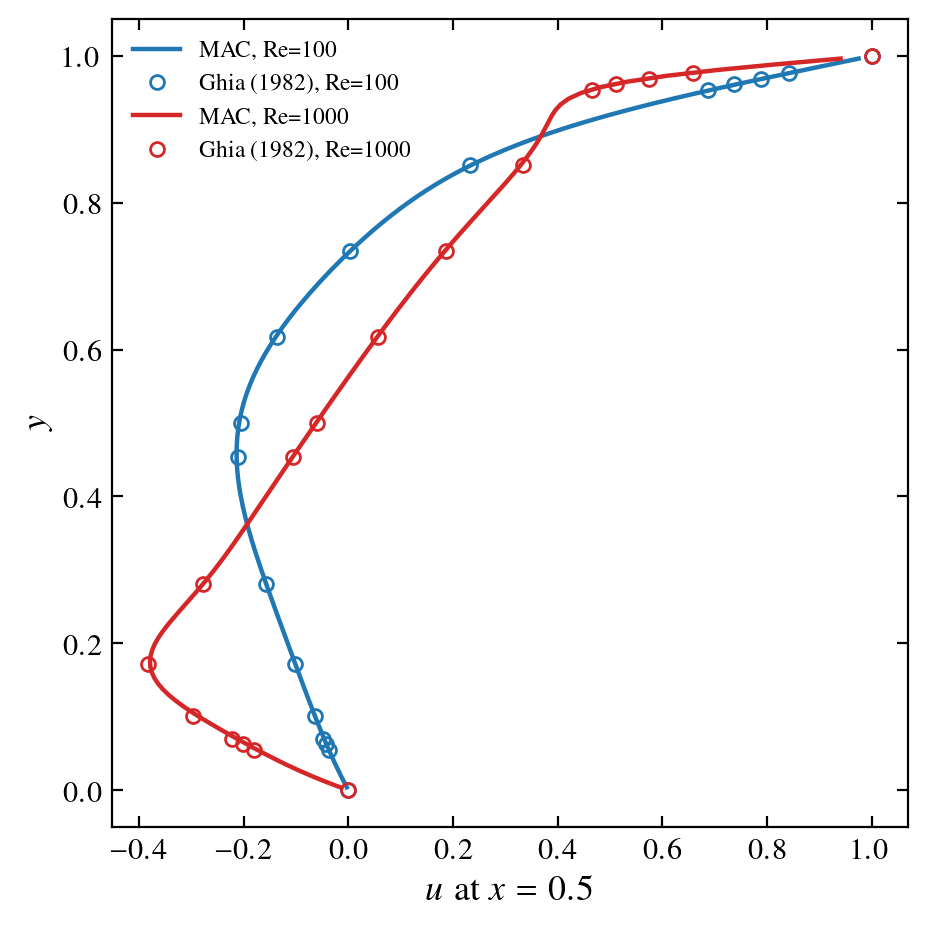
\includegraphics[width=0.47\linewidth]{figures/ghia_uy.png}\hfill
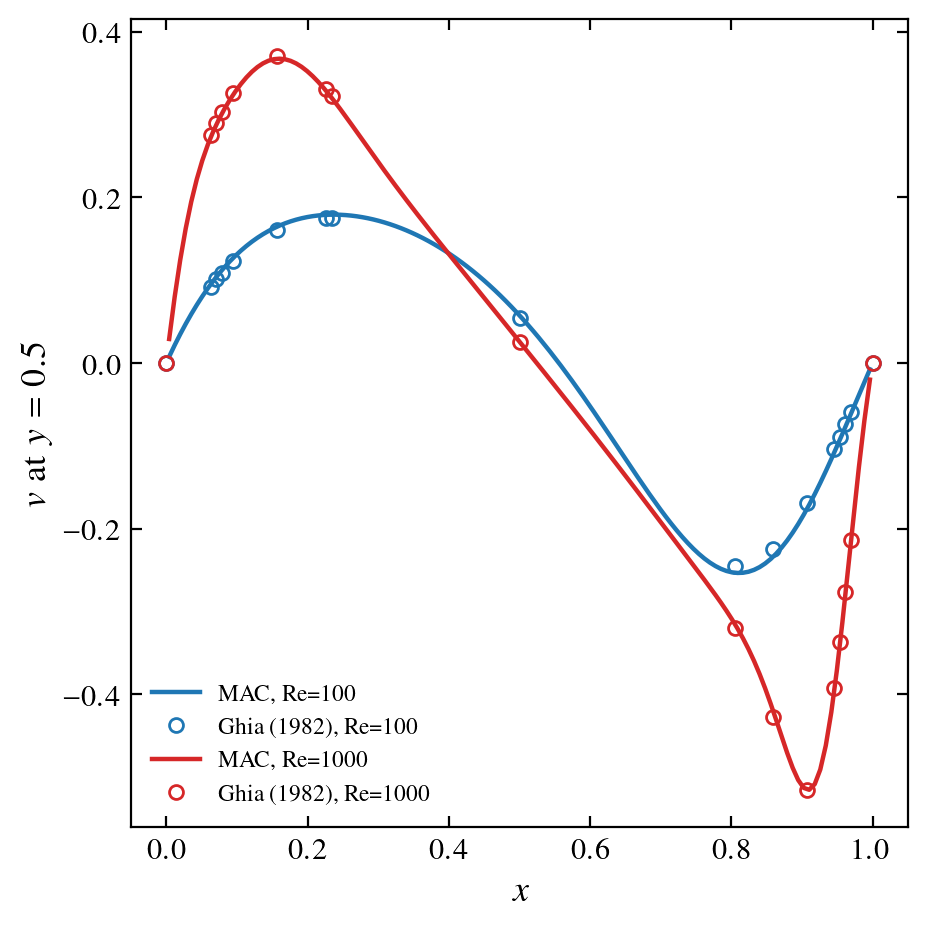
\includegraphics[width=0.47\linewidth]{figures/ghia_vx.png}
\caption{Lid-driven cavity vs.\ Ghia \emph{et al.}\ \cite{Ghia1982} at $\mathrm{Re}=100$ (blue)
and $1000$ (red), $N{=}128$: (left) $u$ on the vertical centreline $x=0.5$; (right) $v$ on the
horizontal centreline $y=0.5$. Lines are the MAC solver; circles the reference.}
\label{fig:ghia}
\end{figure}

\subsection{Developed cavity flow}
The developed (steady) cavity flow at $\mathrm{Re}=100$ and $1000$ ($N{=}128$) is shown in
\cref{fig:lid-developed}: the primary vortex, the secondary corner vortices---stronger and more
extended at $\mathrm{Re}=1000$---and the pressure field, with the low-pressure primary-vortex
core and the high-pressure stagnation region at the top-right corner where the lid drives the
fluid into the wall. Both the streamline topology and the pressure structure are consistent with
the Ghia \emph{et al.}\ benchmark.

\begin{figure}[t]\centering
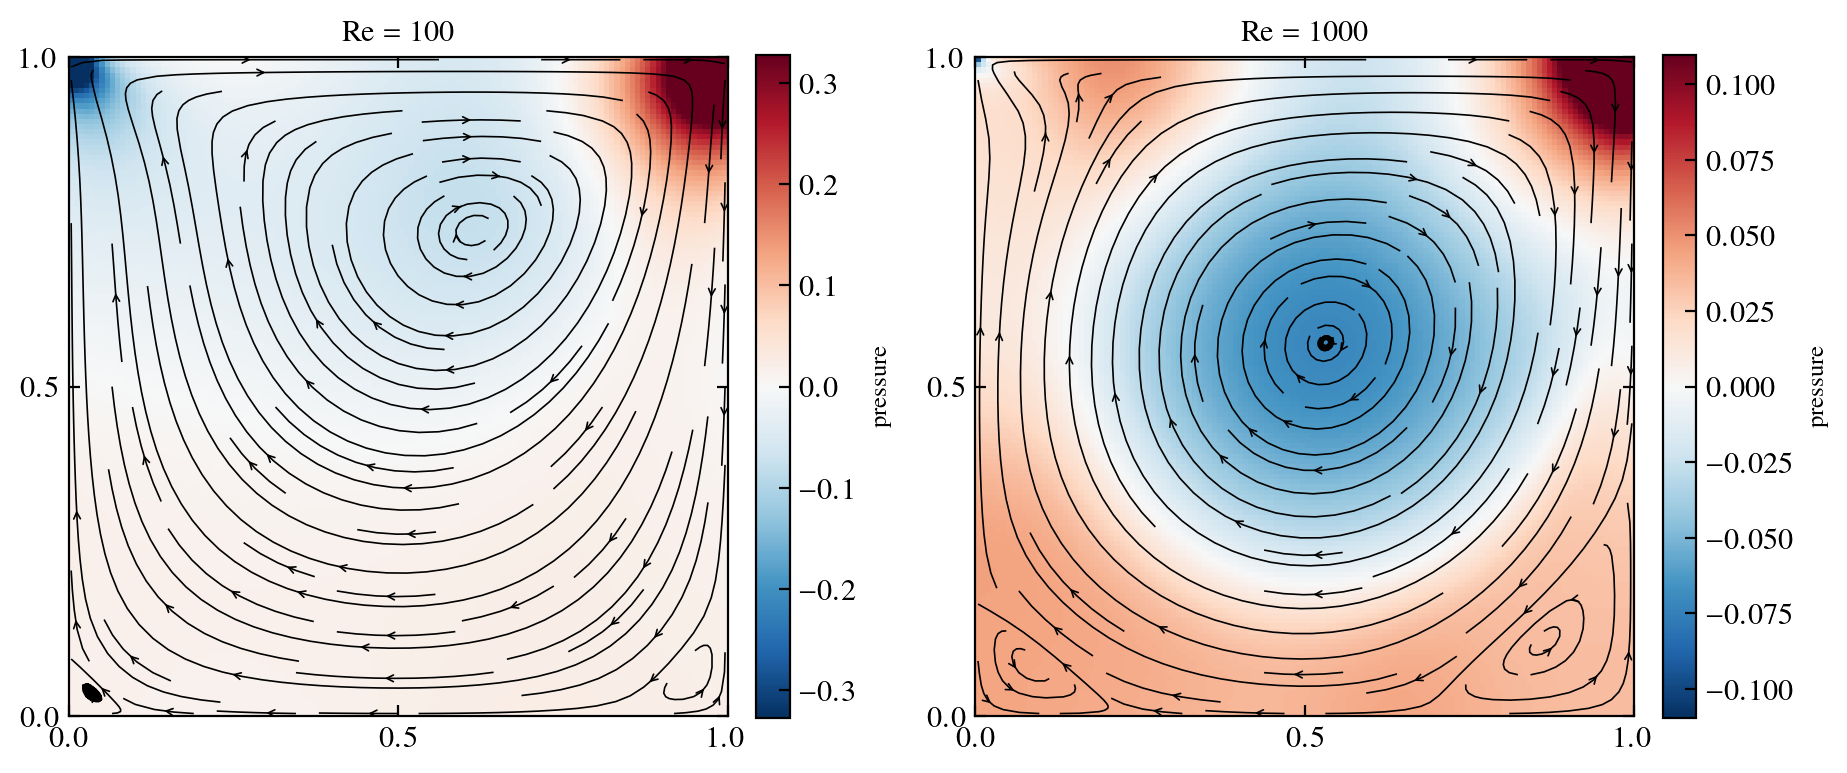
\includegraphics[width=0.9\linewidth]{figures/lid_developed.png}
\caption{Developed lid-driven cavity ($N{=}128$, steady): pressure field (colour) with velocity
streamlines (black), at $\mathrm{Re}=100$ (left) and $1000$ (right). The corner vortices
intensify and the boundary layers thin with Reynolds number.}
\label{fig:lid-developed}
\end{figure}

\section{Reference-map advection: scheme comparison}
\label{sec:supp-advection}
The reference map and log-conformation strain are transported by a monotone bicubic
semi-Lagrangian scheme. \Cref{fig:scheme-compare} shows, on the soft-disc lid-driven cavity
($N{=}128$), that bicubic interpolation tracks the exact Sugiyama $1024^2$ reference around the
entire inward spiral, whereas bilinear interpolation is visibly more diffusive on the inner
turns---the reason the bicubic scheme is the default throughout. The bicubic trajectory is
grid-converged: refining $N{=}128\to256$ shifts it by under $7\times10^{-4}$, so the
${\sim}5\times10^{-3}$ residual to Sugiyama is the scatter of the benchmark itself, not an
under-resolution artifact (main text).

\begin{figure}[t]\centering
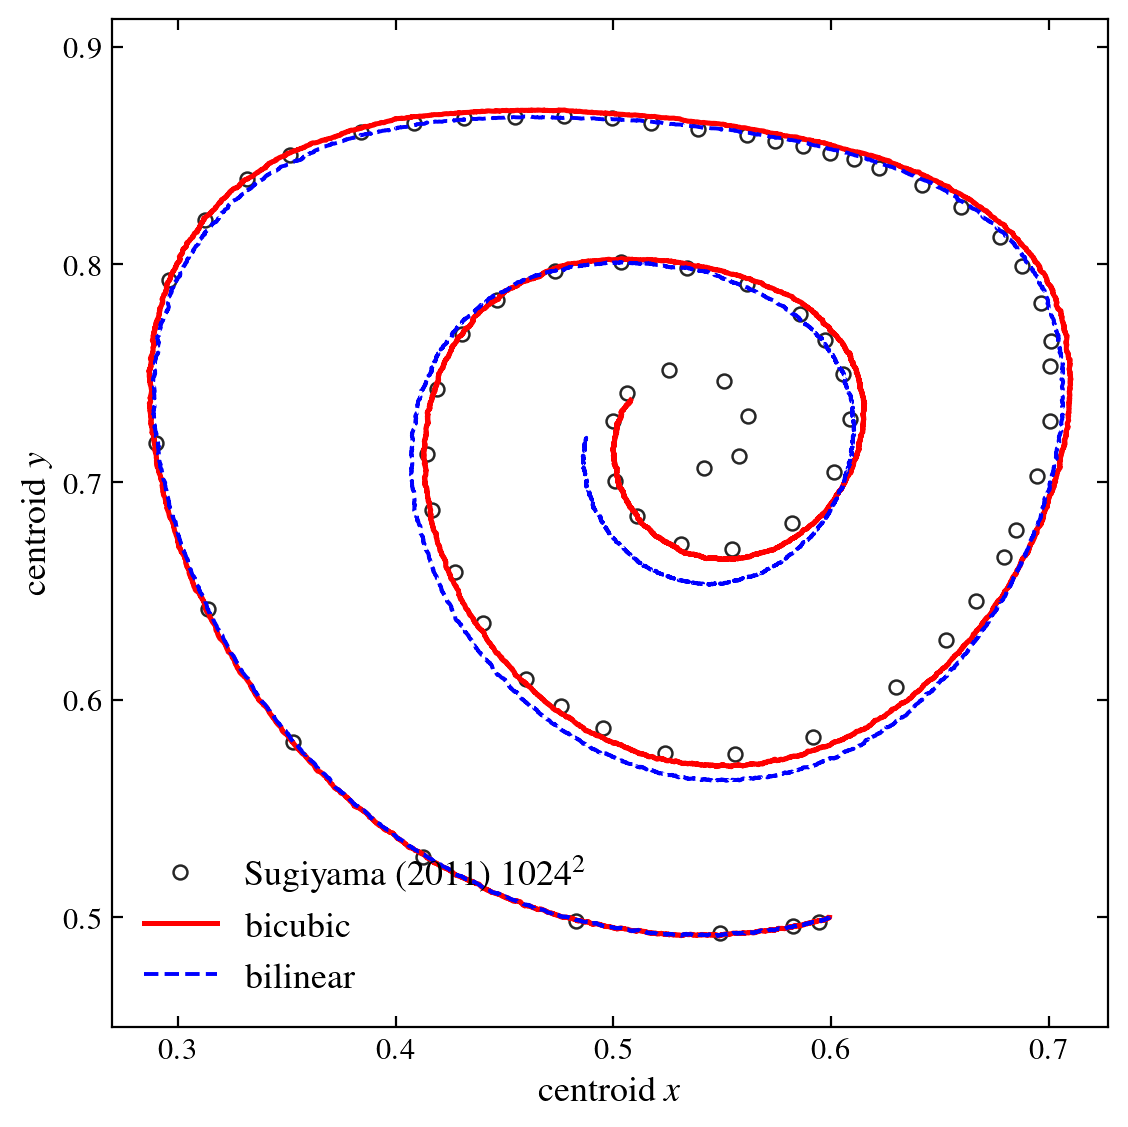
\includegraphics[width=0.5\linewidth]{figures/scheme_compare_N128.png}
\caption{Soft disc in a lid-driven cavity ($N{=}128$): centroid trajectory over the inward
spiral vs.\ the Sugiyama \emph{et al.}\ \cite{Sugiyama2011} $1024^2$ reference. Bicubic
interpolation tracks the reference; bilinear is more diffusive on the inner turns.}
\label{fig:scheme-compare}
\end{figure}

\section{Contact and the elastic-wave stabilizer}
\label{sec:supp-stabilizer}
The explicit baseline and the work--precision/speedup comparison are given in the efficiency
subsection of the main text; here we add the contact-integration detail.
At the colliding-disc parameters the advective and
elastic-wave step limits nearly coincide, so the collisions of the main text are integrated with
the elastic wave resolved (stabilizer off), which keeps the rebound---and hence the coefficient of
restitution---free of numerical damping. Engaging the stabilizer trades that fidelity for
robustness: it damps the under-resolved elastic wave, so IMEX then completes even violent impacts
(e.g.\ $V_0=1.6$, where the forward-Euler elastic force diverges at the same step) but at a lower,
stabilizer-dependent restitution. This is why the stabilizer is reserved for the genuinely stiff
regime (the stiff-solid example of the main text), where stepping past the elastic-wave CFL is the point.

\section{Elastic-wave stabilizer faithfulness}
\label{sec:supp-consistency}
The $\tau\to\infty$ reduction of the viscoelastic model to neo-Hookean elasticity is shown in
the main text; here we check that the elastic-wave stabilizer does not distort the lid-driven
validation. On the elastic ($\tau\to\infty$) disc (Sugiyama parameters, $N{=}128$, bicubic
semi-Lagrangian transport), resolving the elastic wave (stabilizer off, step below the elastic-wave CFL)
reproduces the stabilized run's centroid path to plotting precision (\cref{fig:lid-staboff}),
confirming that the energy-conserving stabilizer is faithful in the regime where it is used.

\begin{figure}[t]\centering
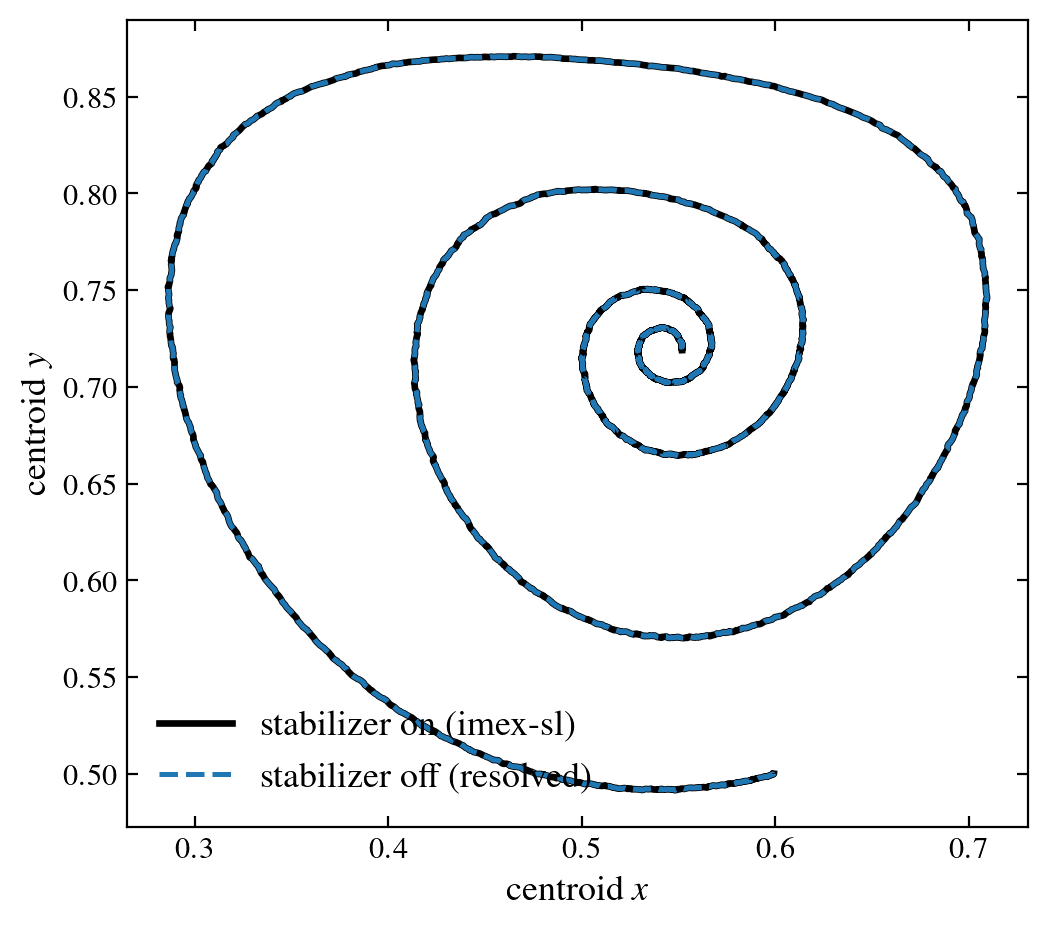
\includegraphics[width=0.5\linewidth]{figures/lid_staboff.png}
\caption{Elastic-wave stabilizer off (dashed) vs.\ on (solid) for the elastic ($\tau\to\infty$) lid-driven
disc: the centroid paths over $t\in[0,24]$ coincide, so the stabilizer does not distort the
trajectory.}
\label{fig:lid-staboff}
\end{figure}

\bibliographystyle{elsarticle-num}
\bibliography{refs}

\end{document}
